\chapter{Theory of Quantum Information and Quantum Network}
\label{theory_of_quantum_information}
\section{History of Quantum Information and Quantum Network}
Quantum computers were proposed by Richard Feynman in 1982\cite{feynman1982simulating}.
It was proposed to simulate quantum systems with a computer based on quantum mechanics since classical computers could not simulate them accurately.
Later, in 1992, the first algorithm for a quantum computer was proposed by Deutsch and Jozsa\cite{deutsch1992rapid}.
In addition, Shor proposed Shor's algorithm for performing factorization in polynomial time\cite{shor1997}, and Grover proposed Grover's algorithm for performing data retrieval in polynomial time\cite{grover1996fast} on a quantum computer.
Currently, research and discussions on quantum computers are very active, and even today, many technologies and new quantum algorithms are being announced for the realization of quantum computers.

On the other hand, along with quantum computers, the field of quantum networks has continued to grow to this day.
In 1984, the first quantum cryptography protocol was proposed by Bennett and Brassard\cite{BEN84}.
This algorithm is called BB84.
This is a famous cryptographic algorithm that uses quantum mechanics, and it has brought quantum mechanics into the spotlight in the field of communications as well.
Shor's algorithm introduced earlier has also attracted attention because of its potential to break the current cryptographic algorithm, the RSA cipher, which is used due to its computational security of prime factorization.
In 1998, the "quantum repeater" was proposed, which is a quantum method of relaying for quantum communications over long distances\cite{briegel1998quantum}\cite{dur1999quantum}.

Currently, there are two main types of quantum networks being actively researched.
The first is called a quantum key distribution network, which uses algorithms such as BB84 and relays classically. 
This type of network is already in the experimental stage on a large scale and is also being used commercially\cite{bennett1992dawn}\cite{elliott2005current}\cite{sasaki2011field}.
The other type of network is called a quantum repeater network.
It is also known as the Quantum Internet.
This is an entanglement-based communication method using the quantum repeater.
Quantum Internet can provide more robust security than quantum key distribution networks, but like quantum computers, there are still many hurdles to overcome before we can use it practically, such as increasing the accuracy of relaying using quantum repeaters.
This project is about the Quantum Internet.

\section{Qubit}
In classical information theory, information is represented by bits.
In quantum information theory, information is represented by Qubit.
A bit can take the value of 0 or 1.
On the contrary, qubit can take on the superposition state of 0 and 1.
While classical bits are implemented by turning on and off voltages, etc., qubits are implemented by quantum states.

\subsection{Dirac Notation}
Dirac notation is a notation for quantum states proposed by Dirac\cite{dirac1939new}.
In Dirac notation, quantum states are represented by column vectors $|\psi\rangle$.
$| \rangle$ is called "ket" and colomun vector is called "statevector".
A single qubit can be represented by a dirac notation as follows,
\begin{equation}
    \label{dirac}
    |\psi\rangle = \alpha |0\rangle + \beta |1\rangle = 
    \begin{pmatrix}
        \alpha \\
        \beta \\
    \end{pmatrix}
\end{equation}

$|\psi\rangle$ is a superposition of $|0\rangle$ and $|1\rangle$.
$|0\rangle$ and $|1\rangle$ are computational basis states and defined as follows,

\begin{equation}
    |0\rangle = 
    \begin{pmatrix}
        1 \\
        0 \\
    \end{pmatrix}
\end{equation}
\begin{equation}
    |1\rangle = 
    \begin{pmatrix}
        0 \\
        1 \\
    \end{pmatrix}
\end{equation}

In equation \ref{dirac}, $\alpha$ and $\beta$ are complex numbers, meaning probability amplitudes.
In simple terms, these numbers represent the probability of convergence to that computational basis.
If you would like to know the probability of convergence to that computational basis, you can calculate it by squaring the probability amplitude.
In other words, the following equation holds in the probability amplitude.

\begin{equation}
    |\alpha|^2 + |\beta|^2 = 1
\end{equation}

In other words, the state of a qubit is a vector in a two-dimensional complex vector space.
$|0\rangle$ and $|1\rangle$ form an orthonormal basis for this vector space\cite{nielsen}.

\section{Multiple Qubit System}
Now, for 2 qubits state $|\psi\rangle$, it can be represented as follows.
\begin{equation}
    |\psi\rangle = \alpha_{00} |00\rangle + \alpha_{01} |01\rangle + \alpha_{10} |10\rangle + \alpha_{11} |11\rangle =
    \begin{pmatrix}
        \alpha_{00} \\
        \alpha_{01} \\
        \alpha_{10} \\
        \alpha_{11} \\
    \end{pmatrix}
\end{equation}
As you can see, there are four computational basis.
The computational basis for $N$ qubits, and the size of the statevector, is $2^N$.
In other words, the space that a qubit can represent increases exponentially.

If you would like to write multiple qubit states from multiple single qubit, you can represent them by taking the tensor product.

\begin{equation}
    |\psi\rangle = |0\rangle \otimes |0\rangle = 
    \begin{pmatrix}
        1 \\
        0 \\
    \end{pmatrix} \otimes
    \begin{pmatrix}
        1 \\
        0 \\
    \end{pmatrix} =
    \begin{pmatrix}
        1 \\
        0 \\
        0 \\
        0 \\
    \end{pmatrix} = |00\rangle
\end{equation}

There are also quantum states that cannot be decomposed and written as independent one-qubit states, as shown below. 

\begin{equation}
    |\psi\rangle = \frac{1}{\sqrt{2}} |00\rangle + \frac{1}{\sqrt{2}} |11\rangle
\end{equation}
Such a state is called "entangled state"(section \ref{entanglement}).

\section{Quantum Gates}
Classical computers have what are called logic gates, and quantum gates are their counterparts.
All quantum gates can be represented by a matrix.
Also, all quantum gates satisfy the unitary matrix, $U^*U = UU^* = I$.
U is the unitary matrix, U* is the adjugate matrix of U, and I is the identity matrix.
Multiple quantum gates can be regarded as a single quantum gate by multiplying them together since they are a matrix.

There are two main types of quantum gates: single qubit gates and controlled gates (multiple qubit gates).

\subsection{Single Qubit Gates}
A single qubit gate is a quantum gate that apply to a single qubit\cite{qgate}.
There are many different types of gates.
\subsection*{X gate(NOT gate)}
X gate (sometimes called the NOT gate) is the NOT gate in classical gates.
\begin{equation}
    X =
    \begin{pmatrix}
        0 & 1\\
        1 & 0\\
    \end{pmatrix}
\end{equation}
This gate flip the bits like the classic NOT gate.
\begin{equation}
    X |0\rangle =
    \begin{pmatrix}
        0 & 1\\
        1 & 0\\
    \end{pmatrix}
    \begin{pmatrix}
        1 \\
        0 \\
    \end{pmatrix} = 
    \begin{pmatrix}
        0 \\
        1 \\
    \end{pmatrix} = |1\rangle
\end{equation}

\subsection*{Z gate(Phase gate)}
Z gate is also called phase gate.
\begin{equation}
    Z =
    \begin{pmatrix}
        1 & 0\\
        0 & -1\\
    \end{pmatrix}
\end{equation}
This gate flip the phase when the qubit is $|1\rangle$.
\begin{equation}
    Z |0\rangle =
    \begin{pmatrix}
        1 & 0\\
        0 & -1\\
    \end{pmatrix}
    \begin{pmatrix}
        1 \\
        0 \\
    \end{pmatrix} = 
    \begin{pmatrix}
        1 \\
        0 \\
    \end{pmatrix} = |0\rangle
\end{equation}
It has no effect in $|0\rangle$.
\begin{equation}
    Z |1\rangle =
    \begin{pmatrix}
        1 & 0\\
        0 & -1\\
    \end{pmatrix}
    \begin{pmatrix}
        0 \\
        1 \\
    \end{pmatrix} = 
    \begin{pmatrix}
        0 \\
        -1 \\
    \end{pmatrix} = -|1\rangle
\end{equation}
In the $|1\rangle$ state, the phase flips so the state to $-|1\rangle$.
\subsection*{Hadamard gate(H gate)}
\begin{equation}
    H = \frac{1}{\sqrt{2}}
    \begin{pmatrix}
        1 & 1\\
        1 & -1\\
    \end{pmatrix}
\end{equation}
This gate is known to be a gate that, when applied to a qubit in the $|0\rangle$ or $|1\rangle$, creates a 50:50 superposition of states.
\begin{equation}
    H |0\rangle =
    \frac{1}{\sqrt{2}}
    \begin{pmatrix}
        1 & 1\\
        1 & -1\\
    \end{pmatrix}
    \begin{pmatrix}
        1 \\
        0 \\
    \end{pmatrix} = 
    \frac{1}{\sqrt{2}}
    \begin{pmatrix}
        1 \\
        1 \\
    \end{pmatrix} =  \frac{|0\rangle + |1\rangle}{\sqrt{2}}
\end{equation}

\subsection*{U gate}
There are other famous single qubit gates as well.
However, there is a constraint that quantum gates are unitary matrices, and we can use this to generalize.
Its generalized single qubit gate is the U gate.
\begin{equation}
    U(\theta, \phi, \lambda) = 
    \begin{pmatrix}
        \cos{\frac{\theta}{2}} & -e^{i\lambda} \sin{\frac{\theta}{2}}\\
        e^{i\lambda} \sin{\frac{\theta}{2}} & e^{i\lambda+i\phi} \cos{\frac{\theta}{2}}\\
    \end{pmatrix}
\end{equation}
U gate requires three parameters: $\theta, \phi, \lambda$.
This gate allows all single qubit gates to be represented.

\subsection{Controlled Gates}
A control gate is a gate that apply to two or more qubits\cite{qgate}.
\subsection*{CNOT (controlled-X) gate}
\begin{equation}
    CNOT = 
    \begin{pmatrix}
        1 & 0 & 0 & 0\\
        0 & 1 & 0 & 0\\
        0 & 0 & 0 & 1\\
        0 & 0 & 1 & 0
    \end{pmatrix}
\end{equation}
The CNOT gate is a gate that causes the second qubit to flip when the first qubit is in the $|1\rangle$ state.
\begin{equation}
    CNOT(\frac{|0\rangle + |1\rangle}{\sqrt{2}}, |0\rangle) = \frac{|00\rangle + |11\rangle}{\sqrt{2}}
\end{equation}
A controlled gate can create an entanglement.

An important element of quantum circuits is that there can be any number of ways to implement the circuit.
A controlled gate has a much higher error rate than a single qubit gate when operated in a real device.
Therefore, one of the challenges for researchers is how to implement the same quantum circuit with fewer controlled gates.

Another important point is that all quantum gates can be decomposed into single qubit gates and CNOT gates.
Since all single qubit gates can be represented by U gates, all quantum circuits can be made with U gates and CNOT gates.
This is equivalent to saying that in classical circuits, all circuits can be made with NAND gates.

\section{Superposition}
\label{superposition}
A superposition is a state unique to quantum states in which $|0\rangle$ and $|1\rangle$ exist simultaneously.
\begin{equation}
    \label{superposition_eq}
    |\psi\rangle =  \frac{1}{\sqrt{2}}|0\rangle + \frac{1}{\sqrt{2}}|1\rangle
\end{equation}
The number in front of the two computational bases is called the probability amplitude and indicates the probability of convergence to that basis when measured.
Superposition is a phenomenon unique to quantum states, and quantum states converge to a single state when measured. 
In other words, in the case of qubits, they converge to 0 or 1.
If you would like to know the probability of convergence, you can calculate it by squaring the probability amplitude.
In equation \ref{superposition_eq}, $(\frac{1}{\sqrt{2}})^2 = \frac{1}{2}$ so the probability of convergence to 0 and 1 is 1/2.
This superposition feature allows a quantum computer to perform calculations in a larger space than a classical computer.
\section{Entanglement}
\label{entanglement}
Entanglement is a quantum state consisting of multiple qubits is a state in which the qubits are not independent and have some quantum mechanical correlation\cite{nielsen}.
If a quantum state consisting of multiple qubits cannot be represented as individual qubits, then those qubits are said to be entangled.
\begin{equation}
    \label{not_entangled}
    |\psi\rangle = \frac{1}{\sqrt{2}} (|00\rangle + |01\rangle)
    = |0\rangle \otimes \frac{1}{\sqrt{2}}(|0\rangle + |1\rangle)
\end{equation}
The quantum state of the equation \ref{not_entangled} is not an entangled state, since it can be split into individual qubits.
\begin{equation}
    \label{entangled}
    |\psi\rangle = \frac{1}{\sqrt{2}} (|00\rangle + |11\rangle)
\end{equation}
The quantum state of the equation \ref{entangled} is an entangled state, since it cannot be split into individual qubits.

The important point of entanglement is that these quantum states are correlated.
For example, if you measure the quantum states of equation \ref{entangled} one qubit at a time, if the first result is zero, the other result will always be zero, and if it is one, the other result will always be one. 
This happens no matter how far apart the two qubits are.

\section{Bell States}
The Bell state is the simplest pair of entanglements in two qubits. 
The following four states are called Bell states.
\begin{equation}
    |\phi^+\rangle = \frac{1}{\sqrt{2}} (|00\rangle + |11\rangle)
\end{equation}
\begin{equation}
    |\phi^-\rangle = \frac{1}{\sqrt{2}} (|00\rangle - |11\rangle)
\end{equation}
\begin{equation}
    |\psi^+\rangle = \frac{1}{\sqrt{2}} (|01\rangle + |10\rangle)
\end{equation}
\begin{equation}
    |\psi^-\rangle = \frac{1}{\sqrt{2}} (|01\rangle - |10\rangle)
\end{equation}

Bell states use as a basis. 
This is called the Bell basis.
Using Bell basis, the computational basis can be written as follows\cite{q-leap_Bell},
\begin{equation}
    |00\rangle = \frac{1}{\sqrt{2}} (|\phi^+\rangle + |\phi^-\rangle)
\end{equation}
\begin{equation}
    |01\rangle = \frac{1}{\sqrt{2}} (|\psi^+\rangle + |\psi^-\rangle)
\end{equation}
\begin{equation}
    |10\rangle = \frac{1}{\sqrt{2}} (|\psi^+\rangle - |\psi^-\rangle)
\end{equation}
\begin{equation}
    |11\rangle = \frac{1}{\sqrt{2}} (|\phi^+\rangle - |\phi^-\rangle)
\end{equation}
Bell basis is used in quantum teleportation and entanglement swapping, which is a technique of quantum repeater\cite{q-leap_Bell}.

\section{Quantum Teleportation}
According to \cite{nielsen},
\begin{quote}
    Quantum teleportation is a technique for moving quantum states around, even in the absence of a quantum communications channel linking the sender of the quantum state to the recipient.
\end{quote}

When people hear the word teleportation, they think of instantaneous travel.
In other words, we would expect objects or information to travel faster than the speed of light!
The entanglement correlation happens no matter how far apart the two qubits are, which makes the expectation even higher.
However, this is not the case with quantum teleportation.
Quantum teleportation requires the transmission of classical information, which of course does not exceed the speed of light.
Therefore, superluminal communication cannot be realized by quantum teleportation.

This section uses an example to explain quantum teleportation. 
The explanation is based on the derivation by \cite{q-leap_teleportation}
Suppose Alice would like to send Bob any one of the following qubits by quantum teleportation.
\begin{equation}
    \label{teleportation:A1}
    |\psi\rangle_{A_1} = \alpha |0\rangle + \beta |1\rangle
\end{equation}
For quantum teleportation to work, Alice and Bob must share the Bell state.
Therefore, it is assumed that the following Bell states are shared.
\begin{equation}
    \label{teleportation:Bell}
    |\phi^+\rangle_{A_2B}  = \frac{1}{\sqrt{2}} (|00\rangle + |11\rangle)
\end{equation}
Let $A_1$ be the qubit that Alice would like to send, $A_2$ be the qubit of one of the Bell states that Alice has, and $B$ be the qubit of one of the Bell states that Bob has.
This is represented in the figure below.
\begin{figure}[H]
    \centering
    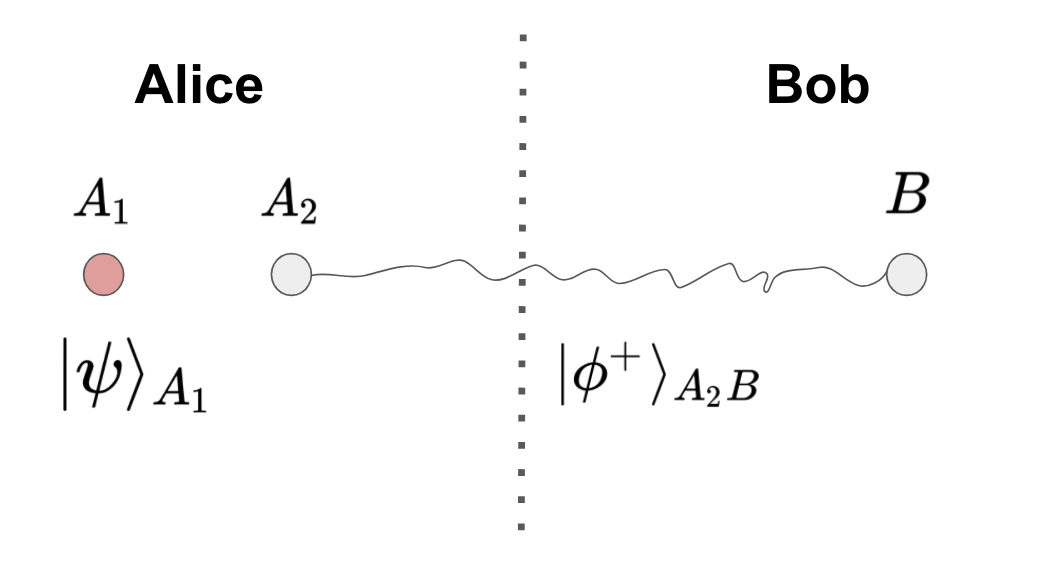
\includegraphics[width=10cm]{img/q-teleportation.png}
    \caption{Quantum Teleportation Example, Alice to Bob}
    \label{fig:teleportation} 
\end{figure}
Equation \ref{teleportation:A1} and \ref{teleportation:Bell} can be combined to be written as follows.
\begin{eqnarray}
    \label{teleportation:combined}
    |\psi\rangle_{A_1} |\phi^+\rangle_{A_2B}  
    & = &(\alpha |0\rangle + \beta |1\rangle)_{A_1} \frac{1}{\sqrt{2}} (|00\rangle + |11\rangle)_{A_2B} \nonumber \\
    & = &\frac{1}{\sqrt{2}} (\alpha |000\rangle + \alpha |011\rangle + \beta |100\rangle + \beta |111\rangle)_{A_1A_2B}
\end{eqnarray}
This is the initial state.
Here, Alice measures $A_1$ and $A_2$ on a Bell basis.
Therefore, let's rewrite equation \ref{teleportation:combined} in Bell basis.
\begin{eqnarray}
    \label{teleportation:combined_bell}
    |\psi\rangle_{A_1} |\phi^+\rangle_{A_2B}  
    & = & \frac{1}{\sqrt{2}} (\alpha |000\rangle + \alpha |011\rangle + \beta |100\rangle + \beta |111\rangle)_{A_1A_2B} \nonumber\\
    & = & \frac{1}{\sqrt{2}} (\alpha (|\phi^+\rangle + |\phi^-\rangle)|0\rangle \nonumber\\
                            &\;& \;+ \alpha (|\psi^+\rangle + |\psi^-\rangle)|1\rangle \nonumber\\
                            &\;& \;+ \beta (|\psi^+\rangle - |\psi^-\rangle)|0\rangle \nonumber\\
                            &\;& \;+ \beta (|\phi^+\rangle - |\phi^-\rangle)|1\rangle)
\end{eqnarray}
This equation \ref{teleportation:combined_bell} can be further rewritten by regrouping it by Bell basis as follows.
\begin{eqnarray}
    \label{teleportation:bell_basis}
    |\psi\rangle_{A_1} |\phi^+\rangle_{A_2B}  
    & = & \frac{1}{\sqrt{2}} (\alpha (|\phi^+\rangle + |\phi^-\rangle)|0\rangle \nonumber\\
                            &\;& \;+ \alpha (|\psi^+\rangle + |\psi^-\rangle)|1\rangle \nonumber\\
                            &\;& \;+ \beta (|\psi^+\rangle - |\psi^-\rangle)|0\rangle \nonumber\\
                            &\;& \;+ \beta (|\phi^+\rangle - |\phi^-\rangle)|1\rangle) \nonumber\\
    & = & \frac{1}{2} (|\phi^+\rangle_{A_1A_2} (\alpha |0\rangle + \beta |1\rangle)_B \nonumber\\
                    &\;& \;+ |\phi^-\rangle_{A_1A_2} (\alpha |0\rangle - \beta |1\rangle)_B \nonumber\\
                    &\;& \;+ |\psi^+\rangle_{A_1A_2} (\alpha |1\rangle + \beta |0\rangle)_B \nonumber\\
                    &\;& \;+ |\psi^-\rangle_{A_1A_2} (\alpha |1\rangle - \beta |0\rangle)_B)
\end{eqnarray}
Therefore, we can see that the state of Bob's qubit changes depending on the results of Alice's Bell state measurement.
However, this can be undone by a simple gate operation with X gate and Z gate as follows.
\begin{eqnarray}
    |\psi\rangle_{A_1} = \alpha |0\rangle + \beta |1\rangle\\
    Z|\psi\rangle_{A_1} = \alpha |0\rangle - \beta |1\rangle\\
    X|\psi\rangle_{A_1} = \alpha |1\rangle + \beta |0\rangle\\
    ZX|\psi\rangle_{A_1} = \alpha |1\rangle - \beta |0\rangle
\end{eqnarray}
This means that Alice has to inform Bob of the results of the Bell state measurement. 
Bob can reproduce the quantum state that Alice would like to send by manipulating the gate according to the results sent by Alice.
This is how information is transmitted via quantum teleportation.
\clearpage
\section{Quantum Network}
\subsection{Quantum Repeater Network}
Quantum repeater network is an entanglement-based communication method using the quantum repeater.
It is also called the Quantum Internet.
Each end node shares a Bell pair and exchanges information through quantum teleportation.

\begin{screen}
Here is Quantum Internetworking flow briefly below.
    \begin{enumerate}
        \item Initiator sends a setup request to responder to share n Bell pairs
        \item Perform an operation to share Bell pairs.
        \item Someone(it depends on link type) sends the result of whether the sharing was a success or failure to the initiator and responder.
    \end{enumerate}
\end{screen}

Entangled states are symmetric so there is no source and destination.
Therefore, there is no such thing as ingress traffic and egress traffic as in the current Internet.
However, there is such a thing as an initiator and a responder in a server-client type application.
This is because when one node starts communication, it needs to send a connection setup request to another node.
The node which sends the connection setup request is called the initiator, and the node which receives the request is called the responder.

\subsection{Quantum Internet Simulator}
Our group, AQUA, has released QuISP, a Quantum Internet simulator. \cite{satoh2021quisp}

However, its functionality is limited so it does not allow us to test traffic using the gravity model, nor does it allow us to connect to multiple nodes or measure traffic.

%%% Local Variables:
%%% mode: japanese-latex
%%% TeX-master: "../thesis"
%%% End: